\documentclass[tikz, border=3mm]{standalone}
\usepackage{tikz}
\usepackage{amsmath} % For \operatorname if needed
\usepackage{amssymb} % For \mathbb
\usetikzlibrary{patterns.meta} % For patterns
\usetikzlibrary{positioning} % Needed for below=... of ...

\begin{document}
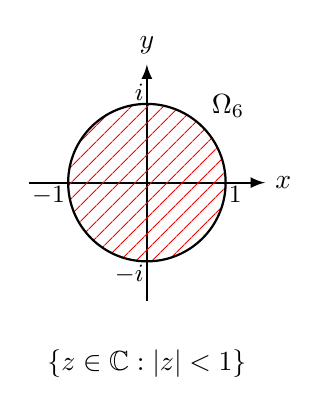
\begin{tikzpicture}[
    % Define axis style
    axis/.style={->, >=latex, thick},
    labelpos/.style={font=\small, inner sep=1pt} % Style for axis intercept labels
]

% Define radius and axis limits
\def\radius{1}
\def\axlim{1.5} % How far the axes should extend

% Axes
\draw[axis] (-\axlim, 0) -- (\axlim, 0) node[right] {$x$};
\draw[axis] (0, -\axlim) -- (0, \axlim) node[above] {$y$};

% Fill the circle with pattern first
\fill[pattern={Lines[angle=45, distance=4pt]}, pattern color=red] (0,0) circle (\radius);

% Draw the circle border on top
\draw[thick] (0,0) circle (\radius);

% Axis Intercept Labels
\node[labelpos, below right] at (\radius, 0) {$1$};
\node[labelpos, below left]  at (-\radius, 0) {$-1$};
\node[labelpos, above left]  at (0, \radius) {$i$};
\node[labelpos, below left]  at (0, -\radius) {$-i$};

% Region Label
\node[above right] at (\radius*0.7, \radius*0.7) {$\Omega_6$};

% Mathematical Description Below
\coordinate (origin) at (0,0);
\node[below=0.5cm of origin, yshift=-\axlim cm] {$\{z \in \mathbb{C} : |z| < 1\}$};

\end{tikzpicture}
\end{document}